\subthesischapter{Comunicación con el pedal motorizado}
Para la comunicación entre los componentes principales de el sistema, juego serio y pedal motorizado, se creó un módulo de comunicación implementado bajo una arquitectura cliente-servidor basada en sockets TCP/IP que garantiza una conexión confiable y efectiva. Este protocolo proporciona una interfaz que utiliza un conjunto de mensajes predefinidos, ver tablas~\ref{table:send-msg-in-game}, \ref{table:recived-msg-in-game}, \ref{table:send-msg-in-calibration}, \ref{table:recive-msg-in-calibration}. El formato de los mensajes sigue una estructura que consta de un encabezado y un cuerpo organizados de la siguiente manera: \#[COMANDO][PARÁMETROS]. El encabezado \underline{COMANDO} indica el tipo de mensaje y el tamaño del cuerpo, lo que facilita la interpretación de los datos recibidos.

Para gestionar la comunicación con el pedal motorizado, se desarrolló un script en C\# llamado \underline{Stream.cs}. Este script utiliza las bibliotecas de .Net\footnote{Entorno de desarrollo de software creado por Microsoft} para establecer y administrar la conexión con el pedal. La comunicación se realiza de manera asíncrona, aprovechando la programación basada en hilos para evitar bloqueos en la aplicación Unity3D mientras se establece la comunica con el dispositivo físico.

% TRAINING : SENT MESSAGES
\begin{table}[ht]
    \centering
    \begin{tabular}{ |c|p{14cm}|}
        \hline
        \multicolumn{2}{|c|}{Entrenamiento: Mensajes enviados} \\
        \hline
        Comandos        &   Descripción \\\hline
        % ----- COMMAND IG -----
        \textbf{ig}     &   \begin{minipage}{14cm}
                                \vspace{2pt}

                                Envía la orden de iniciar las mediciones del juego y sigue el esquema \#ig[modalidad][canal\textsubscript{1}],[canal\textsubscript{2}],[canal\textsubscript{3}],[canal\textsubscript{4}]. Donde:
                                
                                \begin{itemize}
                                    \item \textbf{modalidad} $\in \{0, 1\}$. Se define 0 para la modalidad ligero y 1 para la modalidad clínica.
                                    \item \textbf{canal\textsubscript{i}} $\in \{0, 1\}$. Se define 0 canal no activo y  1 canal activo.  
                                \end{itemize}
                                Ejemplo: \#ig0,1,0,1,1, iniciar juego modalidad ligero con los canales activos 1, 3 y 4.
                                \vspace{2pt}   
                            \end{minipage}\\\hline 
        % ----- COMMAND SG -----
        \textbf{sg}     &   Envía la orden de parar mediciones del juego. \\\hline   
                                
    \end{tabular}
    \caption{Mensajes enviados en el entrenamiento}
    \label{table:send-msg-in-game}
\end{table}

% TRAINING : RECEIVED MESSAGES
\begin{table}[ht]
    \centering
    \begin{tabular}{ |c|p{14cm}|}
        \hline
        \multicolumn{2}{|c|}{Entrenamiento: Mensaje recibido} \\
        \hline
        Comandos        &   Descripción \\\hline
        % ----- COMMAND AR -----
        \textbf{ar}     &   \begin{minipage}{14cm}
                                \vspace{2pt}    
                                Recibe el valor de velocidad angular y de las mediciones de los canales activos, posee el formato. 
                                \#ar[velocidad angular][canal\textsubscript{1}][canal\textsubscript{2}][canal\textsubscript{3}][canal\textsubscript{4}]. 
                                
                                \begin{itemize}
                                    \item Ejemplo: \#ar100,006204511 ... 16038023,
                                \end{itemize}
                                
                                \vspace{2pt}    
                            \end{minipage}\\\hline 
    \end{tabular}
    \caption{Mensaje recibido en el entrenamiento}
    \label{table:recived-msg-in-game}
\end{table}

\newpage
\begin{table}[ht]
    \centering
    \begin{tabular}{ |c|p{14cm}|}
        \hline
        \multicolumn{2}{|c|}{Calibración: Mensajes enviados} \\
        \hline
        Comandos        &   Descripción \\\hline
        % ----- COMMAND CH -----
        \textbf{ch}     &   \begin{minipage}{14cm}
                                \vspace{1pt}
                                Envía la orden de activar o desactivar los canales de mediciones y sigue 
                                el siguiente esquema: \#ch[canal][acción], donde:
                                \begin{itemize}
                                    \item \textbf{canal} $\in \{1,2,3,4\}$. Establece el canal sobre el que se va a realizar la acción.
                                    \item \textbf{acción} $\in \{0, 1\}$. Se define, 0 desactivar canal y 1 activar canal. 
                                \end{itemize}
                                \vspace{1pt}
                            \end{minipage}\\\hline
        % ----- COMMAND IM -----
        \textbf{im}     &   \begin{minipage}{14cm}
                                \vspace{1pt}
                                Envía la orden de iniciar mediciones siguiendo el esquema 
                                \#im[canal\textsubscript{1}][canal\textsubscript{2}][canal\textsubscript{3}][canal\textsubscript{4}]
                                \begin{itemize}
                                    \item canal\textsubscript{i}$\in \{0, 1\}$ , Se define 0 canal no activo y 1 canal activo.
                                \end{itemize}   
                                Ejemplo: \#im1,0,1,0, iniciar medición en los canales 1 y 3.
                                \vspace{1pt}
                            \end{minipage}\\\hline
        % ----- COMMAND LB -----
        \textbf{lb}     &   \begin{minipage}{14cm}
                                \vspace{1pt}
                                Establece las acciones correspondientes al trabajo con la línea base y sigue el siguiente esquema: \#lb[canal][acción], donde:
                                \begin{itemize}
                                    \item \textbf{canal} $\in \{1, 2, 3, 4\}$. Establece el canal sobre el va a realizar la acción.
                                    \item \textbf{acción} $\in \{0, 1, 2, 3, 4\}$ .Establece la acción, esta puede ser: 
                                    \begin{itemize}
                                        \item 0 iniciar iteracción cálculo de línea base.
                                        \item 1 detener iteración cálculo de línea base.
                                        \item 2 aceptar valor de iteracción del cálculo de línea base.
                                        \item 3 rechazar valor de iteracción del cálculo de línea base.
                                        \item 4 obtener valor final de línea base.
                                    \end{itemize}
                                \end{itemize} 
                                \vspace{1pt}
                            \end{minipage}\\\hline
        % ----- COMMAND MCV -----
        \textbf{mc}     &   \begin{minipage}{14cm}
                                \vspace{1pt}
                                Establece las acciones correspondientes al trabajo con la MCV y sigue el siguiente esquema: \#mc[canal][acción], donde:
                                \begin{itemize}
                                    \item \textbf{canal} $\in \{1, 2, 3, 4\}$. Establece el canal sobre el va a realizar la acción.
                                    \item \textbf{acción} $\in \{0, 1, 2, 3, 4\}$ .Establece la acción, esta puede ser: 
                                    \begin{itemize}
                                        \item 0 iniciar iteracción cálculo de MCV.
                                        \item 1 detener iteración cálculo de MCV.
                                        \item 2 aceptar valor de iteracción del cálculo de MCV.
                                        \item 3 rechazar valor de iteracción del cálculo de MCV.
                                        \item 4 obtener valor final de MCV.
                                    \end{itemize}
                                \end{itemize} 
                                \vspace{1pt}
                            \end{minipage}\\\hline
        \textbf{sm}     &   Informa al pedal que se ha llegado al fin de las mediciones. \\\hline               

    \end{tabular}
    \caption{Mensajes enviados en la calibración}
    \label{table:send-msg-in-calibration}
\end{table}  

\begin{table}[ht]
    \centering
    \begin{tabular}{ |c|p{14cm}|}
        \hline
        \multicolumn{2}{|c|}{Calibración: Mensajes recibidos} \\
        \hline
        Comandos        &   Descripción \\\hline
        % ----- COMMAND AR -----
        \textbf{ar}     &   \begin{minipage}{14cm}
                                \vspace{2pt}    
                                Recibe las mediciones de los canales activos, cada medición corresponde con 2 byte de información y se reciben 100 mediciones por cada canal cada 100ms, por lo que cada 400 valores corresponden a las mediciones de los canales del 1 al 4 para ese instante de tiempo.
                                \begin{itemize}
                                    \item Ejemplo: si el primer comando recibido fuese: \#ar031006204511 ... 16038023,
                                \end{itemize}
                                Los dos primeros bytes 03 y 10 corresponden con el valor 0000001100010000$_{B}$ cuyo valor numérico  784 que sería el valor de la EMG para el canal 1 en el milisegundos 1 de la medición.
                                \vspace{2pt}    
                            \end{minipage}\\\hline    
        % ----- COMMAND LB -----         
        \textbf{lb}     &   \begin{minipage}{14cm}
                                \vspace{1pt}
                                Informa a la aplicación del valor de la línea base o iteracción de cálculo de línea base siguiendo el esquema: \#lb[canal][tipo][valor byte 1][valor byte 2] donde:
                                \begin{itemize}
                                    \item \textbf{canal} $\in \{ 1, 2, 3, 4\}$. Establece el canal al que corresponde el valor.
                                    \item \textbf{tipo} $\in \{ 0, 1\}$. Se define 0 si el valor corresponde a un medición de una iteracción o 1 al valor final de la línea base.
                                    \item \textbf{valor} : Son los valores den formato byte del valor de la línea base.  
                                \end{itemize}
                                \vspace{1pt}
                            \end{minipage}\\\hline 
        % ----- COMMAND MC -----                        
        \textbf{mc}     &   \begin{minipage}{14cm}
                                \vspace{1pt}
                                Informa a la aplicación del valor de la MCV o iteracción de cálculo de la MCV siguiendo el esquema: \#mc[canal][tipo][valor byte 1][valor byte 2] donde:
                                \begin{itemize}
                                    \item \textbf{canal} $\in \{ 1, 2, 3, 4\}$. Establece el canal al que corresponde el valor.
                                    \item \textbf{tipo} $\in \{ 0, 1\}$. Se define 0 si el valor corresponde a un medición de una iteracción o 1 al valor final del MCV.
                                    \item \textbf{valor} : Son los valores den formato byte del valor del MCV.  
                                \end{itemize}
                                \vspace{1pt}
                            \end{minipage} \\\hline                        
    \end{tabular}
    \caption{Mensajes recibidos en la calibración}
    \label{table:recive-msg-in-calibration}
\end{table} 

\newpage
\subthesischapter{Ejemplo de comunicación}
En el proceso de calibración mostrado en la figura~\ref{fig: diagram-protocol-in-calibration}  la comunicación inicia con el envío del comando \#ch1,1 correspondiente a la solicitud de activación  del canal1. El envío de mensajes se realiza  a través de funciones específicas para cada tipo de mensaje. Estas funciones serializan tipos de mensajes específicos en un buffer de salida. Una vez codificado el mensaje en el buffer de salida, se llama a la función, \textbf{send\_message()}, que se encarga de enviar el mensaje codificado en el buffer de salida. Según este principio, cada función es responsable de codificar su mensaje respectivo y finalmente enviar el mensaje llamando a la función. Para proteger de escritura simultánea en el buffer de salida por múltiples hilos se usan \textbf{mutexs}\footnote{Mecanismo en el que se intenta dar solución al problema de la sección crítica en un programa.} entre el proceso de serializar el mensaje y el envío por el {\textbf{socket}}\footnote{Canales de comunicación que permiten que procesos no relacionados intercambien datos.}. 
    
A continuación es enviado el mensaje \#im1,0,1,0, para solicitarle al pedal el inicio del proceso de mediciones en los canales 1 y 3  respectivamente, el cual es respondido con una serie de mensajes de la forma \#ar0310 ... 023. La recepción de mensajes está implementada sobre un hilo distinto del principal. Cuando se recibe un mensaje este se almacena en la variable respectiva asociada al tipo de mensaje y se notifica su recepción cambiando una variable de control asociada a la recepción o lanzando un evento para informar al hilo principal de su recepción. Para proteger el acceso a las variables que pueden tener lecturas y escrituras simultáneas por ambos hilos se usan mutexs.

Durante la medición el usuario puede hacer uso de 2 funcionalidades y ejecutarlas en el orden establecido por el protocolo médico, cálculo de la línea base y posteriormente cálculo de la MCV. Ambas funcionalidades pueden repetirse un número indefinido de veces hasta la validación del resultado obtenido. Ejemplo para el cálculo de la línea base:
    
Se envía el mensaje \#lb1,0 para iniciar el cálculo en el canal 1, luego de este es enviado el mensaje  \#lb1,1 para detener el cálculo y esperar respuesta del pedal. La respuesta es enviada bajo el formato  \#lb100310. Por último es enviado el mensaje \#sm para detener la medición y luego \#lb1,2 o \#lb1,3 para aceptar o rechazarlo el valor de iteracción correspondiente.  

\begin{figure}[ht]
    \centering
    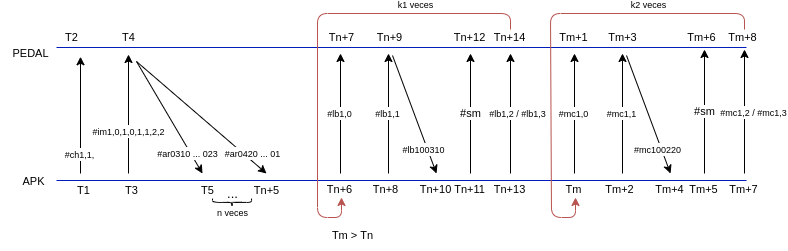
\includegraphics[scale=0.58]{images/diagram-protocol-in-calibration.png}
    \caption{Protocolo de comunicación en la calibración}
    \label{fig: diagram-protocol-in-calibration}
\end{figure}
